\documentclass[border=5pt]{standalone}

\usepackage{amsmath}
\def\pgfsysdriver{pgfsys-dvisvgm.def}
\usepackage{tikz}
\usetikzlibrary{arrows.meta,calc,positioning}

\definecolor{queryblue}{RGB}{210,224,242}
\definecolor{valueorange}{RGB}{247,223,204}
\definecolor{weightblue}{RGB}{232,239,247}
\definecolor{maskgold}{RGB}{247,236,201}
\definecolor{maskgray}{RGB}{150,150,150}
\definecolor{outputgreen}{RGB}{221,236,224}

\tikzset{
  >=Latex,
  flow/.style={->,draw=black,line width=0.7pt},
  flowline/.style={draw=black,line width=0.7pt},
  operator/.style={
    draw=black,
    rectangle,
    minimum height=8.5mm,
    minimum width=18mm,
    inner sep=2pt,
    align=center,
    font=\footnotesize
  },
  circleop/.style={
    draw=black,
    circle,
    minimum size=8.5mm,
    inner sep=0pt,
    font=\small
  },
  dim/.style={font=\scriptsize},
  note/.style={font=\scriptsize,align=center},
  panel/.style={font=\bfseries\large,anchor=west}
}

\newcommand{\gridmatrix}[8]{%
  \begin{scope}[shift={(#1,#2)}]
    \filldraw[fill=#7,draw=black,line width=0.55pt] (0,0) rectangle (#3,#4);
    \pgfmathsetmacro{\colstep}{#3/#6}
    \pgfmathsetmacro{\rowstep}{#4/#5}
    \foreach \col in {1,...,\numexpr#6-1\relax} {
      \draw[line width=0.4pt] (\col*\colstep,0) -- (\col*\colstep,#4);
    }
    \foreach \row in {1,...,\numexpr#5-1\relax} {
      \draw[line width=0.4pt] (0,\row*\rowstep) -- (#3,\row*\rowstep);
    }
    \node[font=\bfseries,above=1.6mm] at (#3/2,#4) {#8};
  \end{scope}
}

\begin{document}
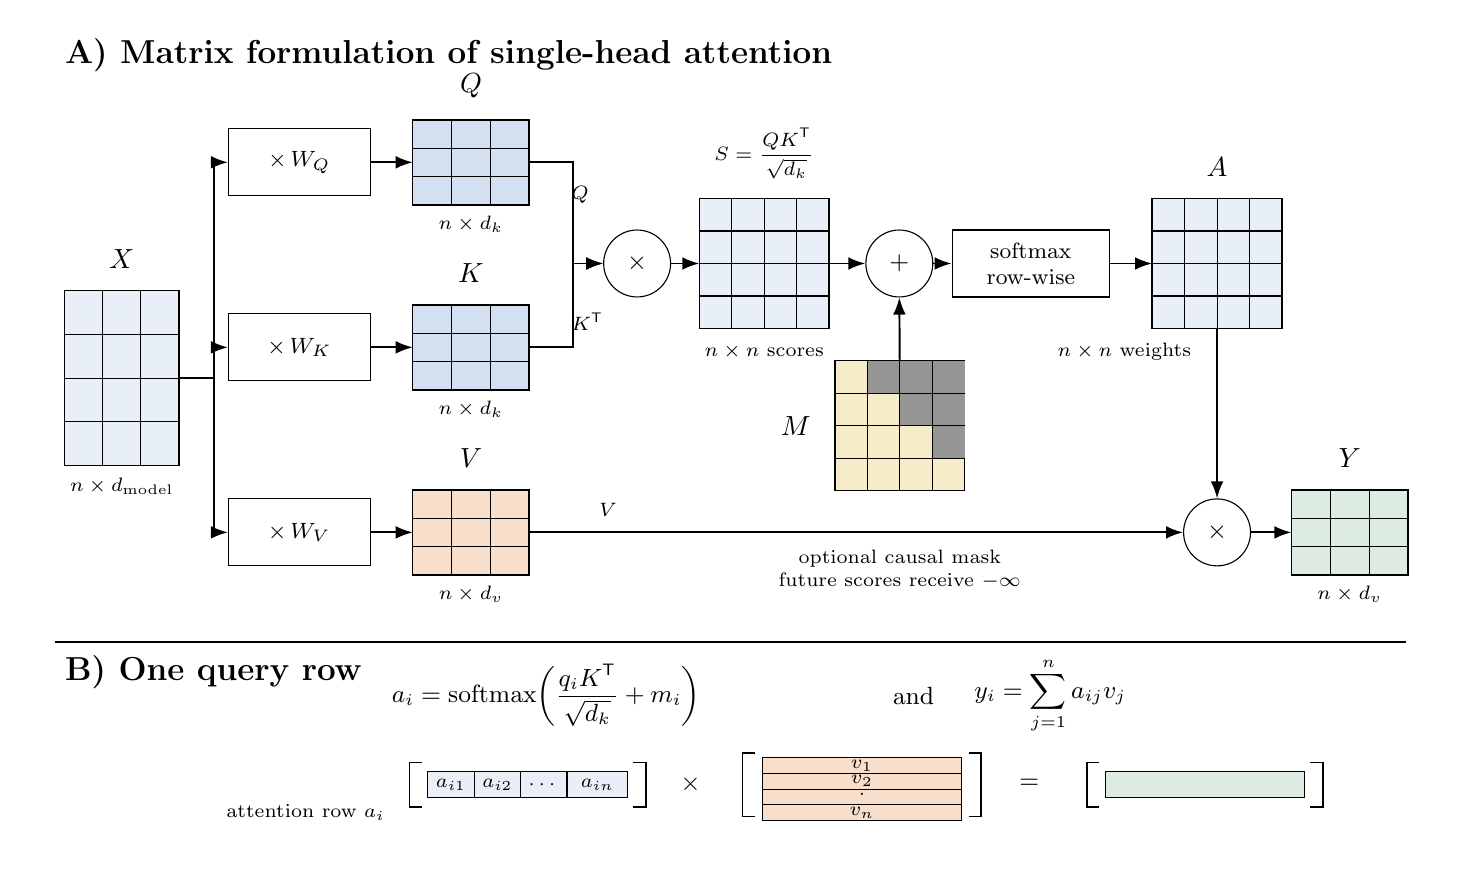
\begin{tikzpicture}[x=1cm,y=1cm]
  \fill[white] (-0.35,-1.70) rectangle (17.55,8.90);

  % Panel A
  \node[panel] at (0,8.55) {A) Matrix formulation of single-head attention};

  % Input and Q/K/V projections
  \gridmatrix{0.12}{3.34}{1.45}{2.22}{4}{3}{weightblue}{$X$}
  \node[dim] (xdim) at (0.845,3.08) {$n \times d_{\mathrm{model}}$};

  \node[operator] (wq) at (3.10,7.19) {$\times\,W_Q$};
  \node[operator] (wk) at (3.10,4.84) {$\times\,W_K$};
  \node[operator] (wv) at (3.10,2.49) {$\times\,W_V$};

  \coordinate (xfan) at (2.02,4.45);
  \draw[flowline] (1.57,4.45) -- (xfan);
  \draw[flowline] (xfan) -- (2.02,7.19);
  \draw[flowline] (xfan) -- (2.02,2.49);
  \draw[flow] (2.02,7.19) -- (wq.west);
  \draw[flow] (2.02,4.84) -- (wk.west);
  \draw[flow] (2.02,2.49) -- (wv.west);

  \gridmatrix{4.54}{6.65}{1.48}{1.08}{3}{3}{queryblue}{$Q$}
  \gridmatrix{4.54}{4.30}{1.48}{1.08}{3}{3}{queryblue}{$K$}
  \gridmatrix{4.54}{1.95}{1.48}{1.08}{3}{3}{valueorange}{$V$}
  \node[dim] at (5.28,6.40) {$n \times d_k$};
  \node[dim] at (5.28,4.05) {$n \times d_k$};
  \node[dim] at (5.28,1.70) {$n \times d_v$};

  \draw[flow] (wq.east) -- (4.54,7.19);
  \draw[flow] (wk.east) -- (4.54,4.84);
  \draw[flow] (wv.east) -- (4.54,2.49);

  % Query-key scores
  \node[circleop] (qkprod) at (7.39,5.905) {$\times$};
  \draw[flow] (6.02,7.19) -- ++(0.55,0) |- (qkprod.west);
  \draw[flow] (6.02,4.84) -- ++(0.55,0) |- (qkprod.west);
  \node[font=\scriptsize,anchor=west] at (6.43,6.78) {$Q$};
  \node[font=\scriptsize,anchor=west] at (6.43,5.17) {$K^{\mathsf T}$};

  \gridmatrix{8.18}{5.08}{1.65}{1.65}{4}{4}{weightblue}{}
  \node[font=\scriptsize,align=center] at (9.005,7.30)
    {$\displaystyle S=\frac{QK^{\mathsf T}}{\sqrt{d_k}}$};
  \node[dim] at (9.005,4.79) {$n \times n$ scores};
  \draw[flow] (qkprod.east) -- (8.18,5.905);

  % Causal mask and row-wise normalization
  \node[circleop] (maskadd) at (10.72,5.905) {$+$};
  \draw[flow] (9.83,5.905) -- (maskadd.west);

  \begin{scope}[shift={(9.90,3.02)}]
    \filldraw[fill=maskgold,draw=black,line width=0.55pt] (0,0) rectangle (1.65,1.65);
    \fill[maskgray] (0.4125,1.2375) rectangle (1.65,1.65);
    \fill[maskgray] (0.825,0.825) rectangle (1.65,1.2375);
    \fill[maskgray] (1.2375,0.4125) rectangle (1.65,0.825);
    \foreach \cell in {1,2,3} {
      \draw[line width=0.4pt] (\cell*0.4125,0) -- (\cell*0.4125,1.65);
      \draw[line width=0.4pt] (0,\cell*0.4125) -- (1.65,\cell*0.4125);
    }
  \end{scope}
  \node[font=\bfseries,anchor=east] at (9.72,3.845) {$M$};
  \node[note] at (10.725,2.02) {optional causal mask\\future scores receive $-\infty$};
  \draw[flow] (10.725,4.67) -- (maskadd.south);

  \node[operator,minimum width=20mm] (softmax) at (12.39,5.905)
    {$\operatorname{softmax}$\\row-wise};
  \draw[flow] (maskadd.east) -- (softmax.west);

  \gridmatrix{13.93}{5.08}{1.65}{1.65}{4}{4}{weightblue}{$A$}
  \node[dim,anchor=east] at (14.55,4.79) {$n \times n$ weights};
  \draw[flow] (softmax.east) -- (13.93,5.905);

  % Attention-weighted value mixing
  \node[circleop] (avprod) at (14.755,2.49) {$\times$};
  \draw[flow] (6.02,2.49) -- (avprod.west);
  \node[font=\scriptsize,anchor=south] at (7.02,2.57) {$V$};
  \draw[flow] (14.755,5.08) -- (avprod.north);

  \gridmatrix{15.70}{1.95}{1.48}{1.08}{3}{3}{outputgreen}{$Y$}
  \node[dim] at (16.44,1.70) {$n \times d_v$};
  \draw[flow] (avprod.east) -- (15.70,2.49);

  % Panel divider
  \draw[line width=0.55pt] (0,1.10) -- (17.15,1.10);

  % Panel B
  \node[panel] at (0,0.72) {B) One query row};
  \node[font=\small,anchor=west] at (4.15,0.42)
    {$\displaystyle a_i=\operatorname{softmax}\!\left(\frac{q_iK^{\mathsf T}}{\sqrt{d_k}}+m_i\right)$};
  \node[font=\small] at (10.90,0.42) {and};
  \node[font=\small,anchor=west] at (11.55,0.42)
    {$\displaystyle y_i=\sum_{j=1}^{n}a_{ij}v_j$};

  \node[font=\scriptsize] at (3.18,-1.07) {attention row $a_i$};
  \draw[line width=0.55pt] (4.66,-1.00) -- (4.50,-1.00) -- (4.50,-0.43) -- (4.66,-0.43);
  \draw[line width=0.55pt] (7.34,-1.00) -- (7.50,-1.00) -- (7.50,-0.43) -- (7.34,-0.43);
  \foreach \leftx/\rightx/\textvalue in {
    4.73/5.32/{a_{i1}},
    5.32/5.91/{a_{i2}},
    5.91/6.50/{\cdots},
    6.50/7.27/{a_{in}}
  } {
    \filldraw[fill=weightblue,draw=black,line width=0.4pt]
      (\leftx,-0.88) rectangle (\rightx,-0.55);
    \node[font=\scriptsize] at ($(\leftx,-0.88)!0.5!(\rightx,-0.55)$) {$\textvalue$};
  }

  \node[font=\small] at (8.07,-0.71) {$\times$};
  \draw[line width=0.55pt] (8.89,-1.12) -- (8.73,-1.12) -- (8.73,-0.31) -- (8.89,-0.31);
  \draw[line width=0.55pt] (11.60,-1.12) -- (11.76,-1.12) -- (11.76,-0.31) -- (11.60,-0.31);
  \foreach \bottom/\top/\textvalue in {
    0.16/0.36/{v_1},
    -0.04/0.16/{v_2},
    -0.24/-0.04/{\vdots},
    -0.44/-0.24/{v_n}
  } {
    \filldraw[fill=valueorange,draw=black,line width=0.4pt]
      (8.98,{\bottom-0.73}) rectangle (11.51,{\top-0.73});
    \node[font=\scriptsize] at (10.245,{(\bottom+\top)/2-0.73}) {$\textvalue$};
  }

  \node[font=\small] at (12.37,-0.71) {$=$};
  \draw[line width=0.55pt] (13.26,-1.00) -- (13.10,-1.00) -- (13.10,-0.43) -- (13.26,-0.43);
  \draw[line width=0.55pt] (15.94,-1.00) -- (16.10,-1.00) -- (16.10,-0.43) -- (15.94,-0.43);
  \filldraw[fill=outputgreen,draw=black,line width=0.4pt]
    (13.34,-0.88) rectangle (15.86,-0.55);
\end{tikzpicture}
\end{document}
